%----------------------------------------------------------------------------
%----------------------------------------------------------------------------
%----------------------------------------------------------------------------
%bb defines the bounding box for the pdf
%viewport defines the area of the pdf used
%in sidewaysfigure the last entry in bb moves the caption toward/away the pic
%in sidewaysfigure the second entry in bb moves the pic toward/away the caption
%----------------------------------------------------------------------------
\begin{figure}
\scalebox{0.8}[0.8]{
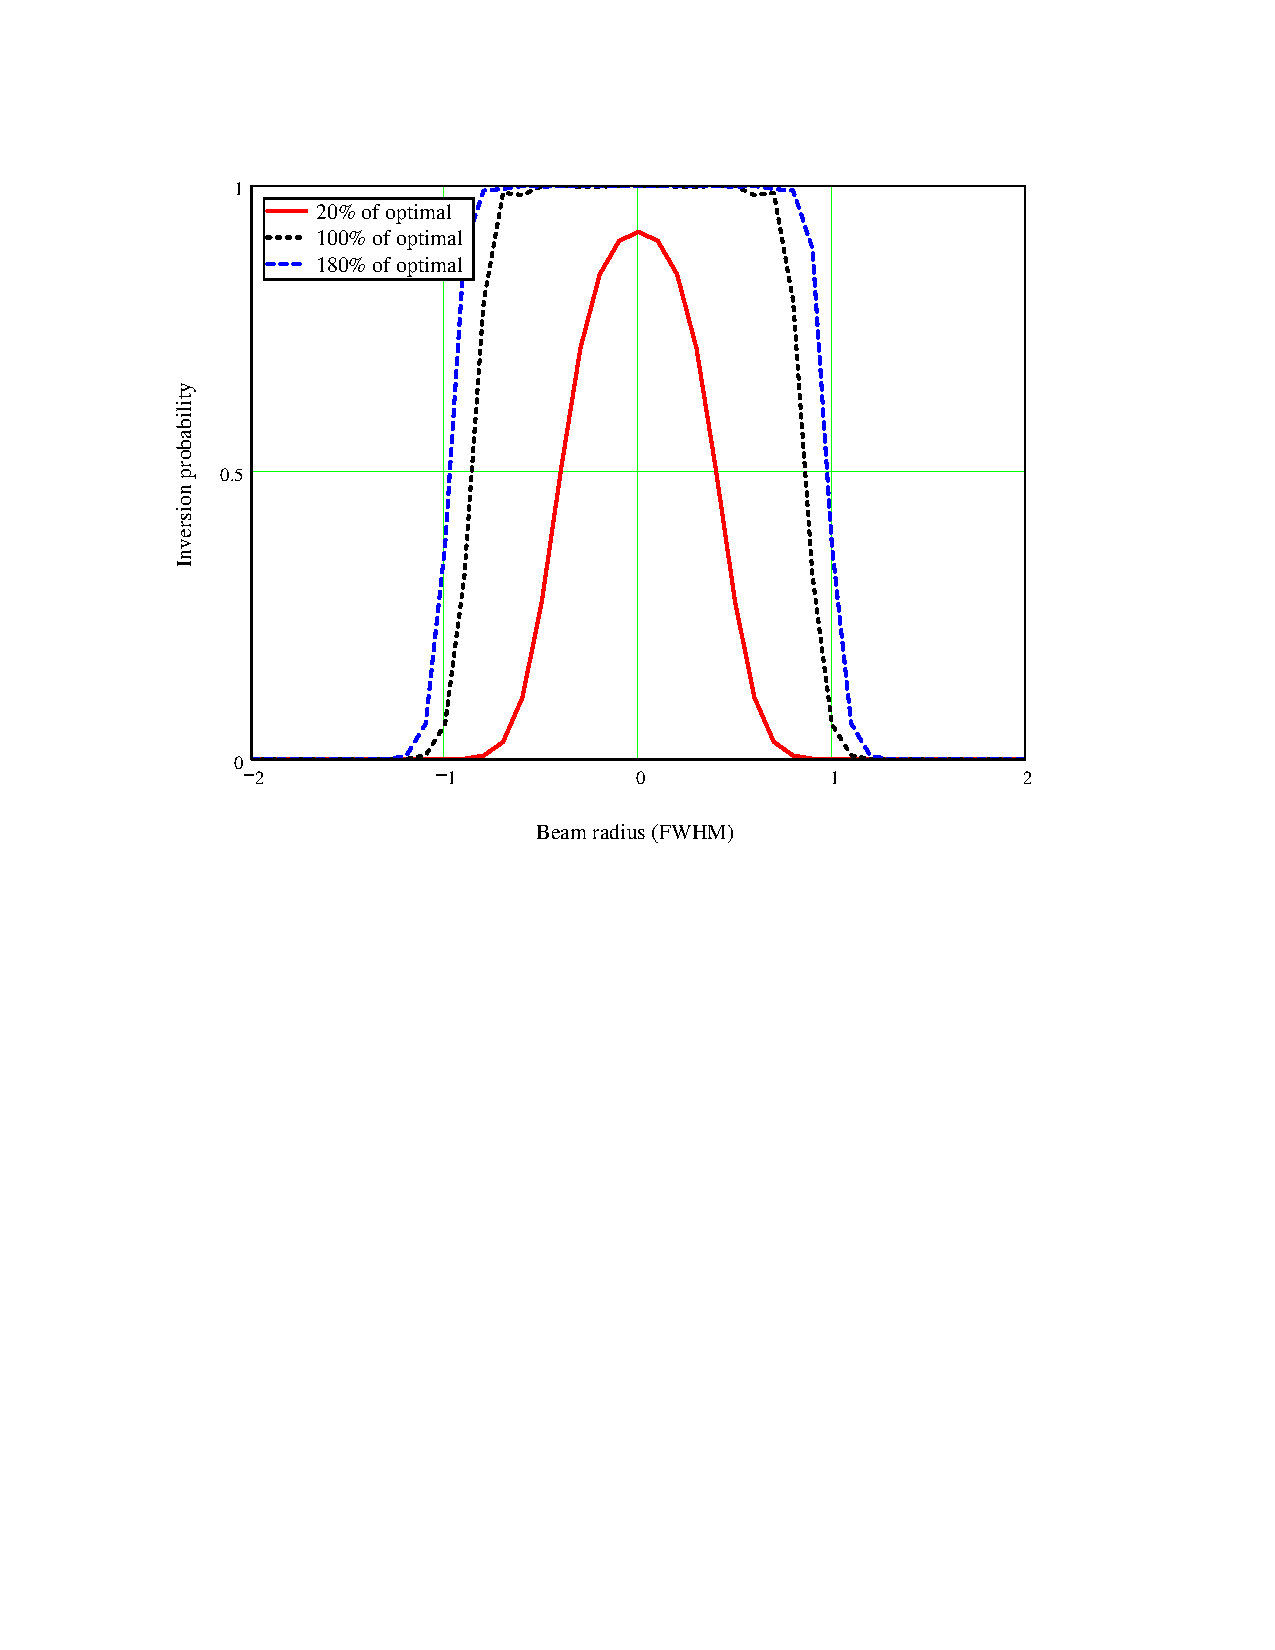
\includegraphics[bb=25 400 489 700]
{gaussian/gaussian.pdf}
}
\caption{Inversion probability across a Gaussian beam profile}
\label{gaussian}
\end{figure}
%----------------------------------------------------------------------------

%----------------------------------------------------------------------------
The STIRAP process also turns out to be beneficial when one considers the spatial distribution of the inverted molecules an a Gaussian beam. The pulse amplitudes are allowed to vary as a pair (the pulses remain of equal height) and the population inversion is calculated across the cross section of Gaussian beam. We see in Figure \ref{gaussian} we see that near top hat cross section are possible.
%----------------------------------------------------------------------------
%----------------------------------------------------------------------------
%----------------------------------------------------------------------------
